% Intended LaTeX compiler: pdflatex
\documentclass[10pt,a4paper,UTF8]{article}
\usepackage{zclorg}
\author{张朝龙}
\date{}
\title{学习Python Doc第五天: 模块}
\hypersetup{
 pdfauthor={张朝龙},
 pdftitle={学习Python Doc第五天: 模块},
 pdfkeywords={},
 pdfsubject={},
 pdfcreator={Emacs 25.0.50.1 (Org mode 9.0.5)}, 
 pdflang={English}}
\begin{document}

\maketitle
\tableofcontents
\titlepic{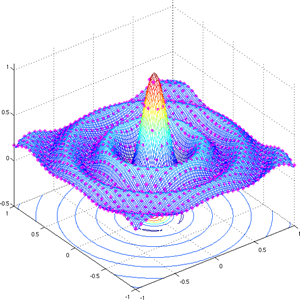
\includegraphics[scale=0.25]{../../img/sinc.PNG}}

\section{简介}
\label{sec:orge2313e9}


如果从 \texttt{Python} 解释器(命令行)退出再进入,那些之前定义的变量,函数都不复存在。如果想保存之前写过的代码,就需要用文件保存起来,下次调用的时候 \texttt{import} 进来。这些保存的文件可以是简单的脚本,亦可是复杂的函数。 \texttt{Python} 把调用的文件叫做 \texttt{module} .一个 \texttt{module} 中的函数定义可以 \texttt{import} 到其他 \texttt{module} 也可以 \texttt{import} 到 \texttt{main module} 

一个 \texttt{module} 包含了 \texttt{Python} 函数定义和语句。这个文件用 \texttt{.py} 作为文件名后缀。 在一个 \texttt{module} 中,  \texttt{module} 的名字是全局变量 \texttt{\_\_name\_\_} 的值。例如,用文本编辑器(推荐 \texttt{vi} 或者 \texttt{Emacs} )创建一个文件命名为 \texttt{fibo.py} 内容是:
\lstset{language=Python,label= ,caption= ,captionpos=b,numbers=none}
\begin{lstlisting}
# Fibonacci numbers module

def fib(n):    # write Fibonacci series up to n
    a, b = 0, 1
    while b < n:
        print(b, end=' ')
        a, b = b, a+b
    print()

def fib2(n):   # return Fibonacci series up to n
    result = []
    a, b = 0, 1
    while b < n:
        result.append(b)
        a, b = b, a+b
    return result
\end{lstlisting}

现在进入 \texttt{Python} 解释器,导入这个 \texttt{modul} 

\begin{verbatim}
>>>import fibo
\end{verbatim}

使用 \texttt{module} 的名字 \texttt{fibo} ,可以调用该 \texttt{module} 中的函数。 比如:
\begin{verbatim}
In [1485]: fibo.fib(1000)
1 1 2 3 5 8 13 21 34 55 89 144 233 377 610 987 

In [1493]: fibo.fib2(100)
Out[1502]: 
[1, 1, 2, 3, 5, 8, 13, 21, 34, 55, 89]
\end{verbatim}

还可以把函数的名字付给一个本地变量:
\begin{verbatim}
In [1503]: fib = fibo.fib

In [1510]: fib(20)
1 1 2 3 5 8 13
\end{verbatim}
\section{深入了解 \texttt{module}}
\label{sec:org921b128}


一个 \texttt{module} 不仅可以包括函数还可以包括可执行语句(由可执行语句集合起来的文件我们也叫脚本)。每一个 \texttt{module} 都有自己的私有符号表,这些符号表对于 \texttt{module} 中的函数来讲是全局的。因此,在 \texttt{module} 中使用全局变量不用担心与另一个人的全局变量产生冲突。

\texttt{module} 可以 \texttt{import} 其他的 \texttt{module} 还可以只调用 \texttt{module} 内的某些名字。

\begin{verbatim}
>>> from fibo import fib,fib2
>>> fib(500)
1 1 2 3 5 8 13 21 34 55 89 144 233 377
\end{verbatim}
这样不会导入模块名,在上面的例子中 \texttt{fibo} 就没有被定义。

可以使用 \texttt{*} 来导入当前 \texttt{module} 中的所有名字:
\begin{verbatim}
>>> from fibo import *
>>> fib(500)
1 1 2 3 5 8 13 21 34 55 89 144 233 377
\end{verbatim}
上面的语句导入了除以下划线开头的所有名字。当然大多数时候,不建议使用这样的做法,因为这样子有可能会导入一些未知的名字进来,有可能会覆盖掉我们自己定义的函数或者变量。另外使用 \texttt{*} 会降低代码的可读性。

注意:从效率方面考虑,每一个 \texttt{module} 都只被导入一次,因此,如果 \texttt{module} 有所改变,你要么重启解释器,要么使用 \texttt{importlib.reload()} 比如: 
\begin{verbatim}
import importlib;
importlib.reload(modulename)
\end{verbatim}

\section{把 \texttt{module} 当做脚本执行}
\label{sec:org4b564c7}


把一个 \texttt{module} 当做脚本执行很简单:
\begin{verbatim}
python fibo.py <arguments>
\end{verbatim}

这个 \texttt{module} 中的代码就会被执行(就像你 \texttt{import} 了它一样),在执行的过程中 \texttt{\_\_name\_\_} 被设置为 \texttt{\_\_main\_\_} ,这意味着通过在 \texttt{module} 的尾部添加,如下语句,就可以把一个 \texttt{module} 当做脚本来使用:
\lstset{language=Python,label= ,caption= ,captionpos=b,numbers=none}
\begin{lstlisting}
if __name__ == "__main__":
    import sys
    fib(int(sys.argv[1]))
\end{lstlisting}

使用过程为:
\begin{verbatim}
>>>python fibo.py 50
1 1 2 3 5 8 13 21 34
\end{verbatim}

\section{\texttt{module} 的搜索路径}
\label{sec:orge969924}


\texttt{import} 一个名称为 \texttt{spam} 的 \texttt{module} 后,解释器首先在内置 \texttt{module} 中搜索 \texttt{spam} 。如果没有找到,然后搜索名字为 \texttt{spam.py} 的文件名,搜索路径为 \texttt{sys.path} 

初始的 \texttt{sys.path} 包含:
\begin{enumerate}
\item 当前路径;
\item \texttt{PYTHONPATH}
\item 安装的默认路径
\end{enumerate}

初始化之后, \texttt{Python} 程序可以修改 \texttt{sys.path} 。包含当前脚本的路径被放在搜索路径的最开始位置(比标准库路径还要靠前),这意味着在当前路径匹配的 \texttt{module} 名会优先被调用。

\section{“编译” \texttt{Python} 文件}
\label{sec:orgfa198a3}


为了加速 \texttt{module} 载入, \texttt{Python} 会把每一个 \texttt{module} 的编译版本 \texttt{module.version.pyc} 放到 \texttt{\_\_pycache\_\_} 目录下。比如,在 \texttt{CPython3.3} 中, \texttt{spam.py} 的编译版本保存路径是 \texttt{\_\_pycache\_\_/spam.cpython-33.pyc} . \texttt{Python} 会像 \texttt{make} 一样自动检测 \texttt{.pyc} 和 \texttt{py} 的时间,然后判断哪些文件需要重新编译。

你可以使用 \texttt{-O} 或者 \texttt{-OO} 选项来让 \texttt{Python} 减小编译文件的大小。 \texttt{-O} 参数移除了 \texttt{assert} 语句。 使用 \texttt{-OO} 参数时,会从字节码中去除 \texttt{\_\_doc\_\_} 以产生更紧凑的 \texttt{.pyo} .

\section{标准模块}
\label{sec:orgdc23d25}


\texttt{Python} 自带了一个标准模板库 \texttt{Python Library Reference} 。一些 \texttt{module} 内置于解释器中,这些 \texttt{module} 提供了 \texttt{Python} 语言核心不提供的功能,比如系统调用;比如 \texttt{winreg}  模块只在Windows上提供。

有一个特殊的模块需要注意 \texttt{sys} 。这个模块内置于所有的 \texttt{Python} 解释器中。比如 变量 \texttt{sys.ps1} 和 \texttt{sys.ps2} 定义了主和次提示符的字符串:

\begin{verbatim}
>>> import sys
>>> sys.ps1
'>>> '
>>> sys.ps2
'... '
>>> sys.ps1 = 'C> '
C> print('Yuck!')
Yuck!
C>
\end{verbatim}

只有解释器处于交互模式时,这两个变量才有意义。

\texttt{sys.path} 包含了解释器搜索 \texttt{module} 的所有路径。可以使用标准的 \texttt{list} 操作符来改变这个值:
\begin{verbatim}
>>> import sys
>>> sys.path.append('/ufs/guido/lib/python')
\end{verbatim}
\section{\texttt{dir()} 函数}
\label{sec:org64897ed}


内置的 \texttt{dir()} 用于找出一个模块里定义了那些名字. 它返回一个有序字串列表:
\begin{verbatim}
>>> import fibo, sys
>>> dir(fibo)
['__name__', 'fib', 'fib2']
>>> dir(sys)  
['__displayhook__', '__doc__', '__excepthook__', '__loader__', '__name__',
 '__package__', '__stderr__', '__stdin__', '__stdout__',
 '_clear_type_cache', '_current_frames', '_debugmallocstats', '_getframe',
 '_home', '_mercurial', '_xoptions', 'abiflags', 'api_version', 'argv',
 'base_exec_prefix', 'base_prefix', 'builtin_module_names', 'byteorder',
 'call_tracing', 'callstats', 'copyright', 'displayhook',
 'dont_write_bytecode', 'exc_info', 'excepthook', 'exec_prefix',
 'executable', 'exit', 'flags', 'float_info', 'float_repr_style',
 'getcheckinterval', 'getdefaultencoding', 'getdlopenflags',
 'getfilesystemencoding', 'getobjects', 'getprofile', 'getrecursionlimit',
 'getrefcount', 'getsizeof', 'getswitchinterval', 'gettotalrefcount',
 'gettrace', 'hash_info', 'hexversion', 'implementation', 'int_info',
 'intern', 'maxsize', 'maxunicode', 'meta_path', 'modules', 'path',
 'path_hooks', 'path_importer_cache', 'platform', 'prefix', 'ps1',
 'setcheckinterval', 'setdlopenflags', 'setprofile', 'setrecursionlimit',
 'setswitchinterval', 'settrace', 'stderr', 'stdin', 'stdout',
 'thread_info', 'version', 'version_info', 'warnoptions']
\end{verbatim}

如果没哟输入参数 \texttt{dir()} 列出了目前你定义的所有名字。 \texttt{dir()} 不会列举所有内置函数和变量,如果你想要看看  \texttt{builtins} 都内置了哪些函数和变量。你可以使用:

\begin{verbatim}
>>> import builtins
>>> dir(builtins)  
['ArithmeticError', 'AssertionError', 'AttributeError', 'BaseException',
 'BlockingIOError', 'BrokenPipeError', 'BufferError', 'BytesWarning',
 'ChildProcessError', 'ConnectionAbortedError', 'ConnectionError',
 'ConnectionRefusedError', 'ConnectionResetError', 'DeprecationWarning',
 'EOFError', 'Ellipsis', 'EnvironmentError', 'Exception', 'False',
 'FileExistsError', 'FileNotFoundError', 'FloatingPointError',
 'FutureWarning', 'GeneratorExit', 'IOError', 'ImportError',
 'ImportWarning', 'IndentationError', 'IndexError', 'InterruptedError',
 'IsADirectoryError', 'KeyError', 'KeyboardInterrupt', 'LookupError',
 'MemoryError', 'NameError', 'None', 'NotADirectoryError', 'NotImplemented',
 'NotImplementedError', 'OSError', 'OverflowError',
 'PendingDeprecationWarning', 'PermissionError', 'ProcessLookupError',
 'ReferenceError', 'ResourceWarning', 'RuntimeError', 'RuntimeWarning',
 'StopIteration', 'SyntaxError', 'SyntaxWarning', 'SystemError',
 'SystemExit', 'TabError', 'TimeoutError', 'True', 'TypeError',
 'UnboundLocalError', 'UnicodeDecodeError', 'UnicodeEncodeError',
 'UnicodeError', 'UnicodeTranslateError', 'UnicodeWarning', 'UserWarning',
 'ValueError', 'Warning', 'ZeroDivisionError', '_', '__build_class__',
 '__debug__', '__doc__', '__import__', '__name__', '__package__', 'abs',
 'all', 'any', 'ascii', 'bin', 'bool', 'bytearray', 'bytes', 'callable',
 'chr', 'classmethod', 'compile', 'complex', 'copyright', 'credits',
 'delattr', 'dict', 'dir', 'divmod', 'enumerate', 'eval', 'exec', 'exit',
 'filter', 'float', 'format', 'frozenset', 'getattr', 'globals', 'hasattr',
 'hash', 'help', 'hex', 'id', 'input', 'int', 'isinstance', 'issubclass',
 'iter', 'len', 'license', 'list', 'locals', 'map', 'max', 'memoryview',
 'min', 'next', 'object', 'oct', 'open', 'ord', 'pow', 'print', 'property',
 'quit', 'range', 'repr', 'reversed', 'round', 'set', 'setattr', 'slice',
 'sorted', 'staticmethod', 'str', 'sum', 'super', 'tuple', 'type', 'vars',
 'zip']
\end{verbatim}
\section{包 ( \texttt{Packages} )}
\label{sec:orgac16391}


包是一种 \texttt{Python}  模块组织命名空间的方法。比如模块名 \texttt{A.B} 是指在包 \texttt{A} 中字块 \texttt{B} 。就像模块的使用,使不同模块的作者不用担心其它全局变量的名字, 而带点号的模块使得多模块包, 例如 NumPy 或 Python 图像库, 的作者不用担心与其他模块名冲突。

假设你想设计一个模块集 (一个 “包”), 用于统一声音文件和声音数据的处理. 有许多不同的声音格式 (通常通过它们的后缀来辨认, 例如: .wave, .aiff, .au), 因此你可能需要创建和维护一个不断增长的模块集, 用以各种各样的文件格式间的转换. 还有许多你想对声音数据执行的不同操作 (例如混频, 增加回音, 应用一个均衡器功能, 创建人造的立体声效果), 因此, 你将额外的写一个永无止尽的模块流来执行这些操作. 这是你的包的一个可能的结构:

\begin{verbatim}
sound/                          Top-level package
      __init__.py               Initialize the sound package
      formats/                  Subpackage for file format conversions
              __init__.py
              wavread.py
              wavwrite.py
              aiffread.py
              aiffwrite.py
              auread.py
              auwrite.py
              ...
      effects/                  Subpackage for sound effects
              __init__.py
              echo.py
              surround.py
              reverse.py
              ...
      filters/                  Subpackage for filters
              __init__.py
              equalizer.py
              vocoder.py
              karaoke.py
              ...
\end{verbatim}

导入一个包时, \texttt{Python} 通过搜索 \texttt{sys.path} 来找包的子目录。

使用 \texttt{\_\_init\_\_.py} 来告诉 \texttt{Python} 哪些目录包含了包。这用来避免名字为一个通用名字(比如 \texttt{string} ), 的目录意外地隐藏了在模块搜索路径靠后的合法模块. 在最简单的例子里,  \texttt{\_\_init\_\_.py}  是个空文件, 但它也可以为这个包执行初始化代码.

使用包可以导入单个模块:
\begin{verbatim}
import sound.effects.echo
\end{verbatim}

这样导入了子模块 \texttt{sound.effects.echo} 。在使用这个子模块时必须使用全名,比如:
\begin{verbatim}
sound.effects.echo.echofilter(input, output, delay=0.7, atten=4)
\end{verbatim}

显然,这很啰嗦。一种简单的调用方法是:
\begin{verbatim}
from sound.effects import echo
\end{verbatim}

调用时,不需要很长的前缀,
\begin{verbatim}
echo.echofilter(input, output, delay=0.7, atten=4)
\end{verbatim}

虽然简单,但是不够简单,我们想要的是 \texttt{foo(a,b,c)} 这样的形式, 看代码:
\begin{verbatim}
from sound.effects.echo import echofilter
\end{verbatim}

调用:
\begin{verbatim}
echofilter(input, output, delay=0.7, atten=4)
\end{verbatim}

现在,我开心了。

通过上面的各种导入过程,我们发现,使用 \texttt{from package import item} 这样的语法 \texttt{item} 可以是一个子模块,也可以是一个包,也可以是一个包中定义的函数。

相反,使用 \texttt{import item.subitem.subsubitem} 每一个项除了最后一个都应该是一个 \texttt{package} ,最后一项必须是 \texttt{module} 或者一个 \texttt{package} 但不许是函数或者变量。

\section{从 \texttt{package} 导入 \texttt{*}}
\label{sec:org3edde7a}


试想 \texttt{from sound.effects import *} 会发生什么?我们希望这句话能够去文件系统中找到所有包中包含的子模块,然后导入。但是这样操作一方面耗时,另一方面有可能出现名字覆盖。

包作者唯一能做的是提供包的显示索引。 \texttt{import} 语句有以下约定:
\begin{enumerate}
\item 如果一个包的 \texttt{\_\_init\_\_.py} 中定义了一个名为 \texttt{\_\_all\_\_} 的列表
\item 当遇到 \texttt{from package import *} 时,它会被用来作为导入的模块名字的列表。
\end{enumerate}

是否维护 \texttt{\_\_all\_\_} 这个变量取决于包作者。例如 \texttt{sound/effects/\_\_init\_\_.py} 可能包含:
\begin{verbatim}
__all__ = ["echo","surround","reverse"]
\end{verbatim}

那么, \texttt{from sound.effects import *} 将导入 \texttt{"echo","surround","reverse"} 这几个子模块。一个放之四海而皆准的导入方法是: \texttt{from package import specific\_submodule} .

\section{包之间的调用}
\label{sec:org07af38b}


当我们需要调用子包内部的模块式,我们实用绝对路径,比如如果 \texttt{sound.filters.vocoder} 需要用到 \texttt{sound.effects} 中的 \texttt{echo} 模块,可以使用:
\begin{verbatim}
from sound.effects import echo
\end{verbatim}

当然也可以使用相对路径来调用,比如 从 \texttt{surround} 模块,可以使用:
\begin{verbatim}
from . import echo
from .. import formats
from ..filters import equalizer
\end{verbatim}

注意相对路径只适合于当前模块。由于主模块的名字永远是 \texttt{\_\_main\_\_} 因此所有需要被当做主模块使用的模块都必须使用绝对路径导入。
\section{在多个文件夹下的包}
\label{sec:org2908df0}


包支持一个特殊的属性 \texttt{\_\_path\_\_} ,这个属性初始化值是一个包含了包含了 \texttt{\_\_init\_\_.py} 目录的名字。可以修改这个变量使得在搜索模块或者子包时查找特定的路径。当然这个属性用的并不经常,主要用这个属性扩展当前包可以调用的模块。
\end{document}
